%%% Time-stamp: <mainrep.tex 19:57, 17 Jul 2016 by P Sunthar>
%%% $Log:$
% This document describes how to use iitbreport style
%********************************************************************

%\documentclass[11pt,a4paper,openright]{report}
\documentclass[twoside]{iitbreport}
%\documentclass[12pt]{article}

%% Default spacing: 1.5
%% Default font size: 12pt
%% Default font: txfonts (similar to times new roman) 

%% Selectively comment out sections that you want to be left out but
%% maintaining the page numbers and other \ref
%\includeonly{
%  intro/introduction,
%  lit/literature,
%  expt/experimental,
%  rnd/results, 
%  dec,abs,pub,ack
%}


%%% Some commonly used packages (make sure your LaTeX installation
%%% contains these packages, if not ask your senior to help installing
%%% the packages)\\

\usepackage{booktabs}

\usepackage{graphicx}
\usepackage{epstopdf}
\usepackage[export]{adjustbox}
\usepackage{caption}
\usepackage{amsmath}
\let\openbox\relax
\usepackage{amsthm}
\usepackage{amssymb}
\usepackage{mathtools}
\usepackage{algorithm}
\usepackage{algorithmic}
\usepackage{amsfonts}
\usepackage[utf8]{inputenc}
\usepackage{lscape}
\usepackage{afterpage}
\allowdisplaybreaks

\makeatletter
\newcommand*\bigcdot{\mathpalette\bigcdot@{1}}
\newcommand*\bigcdot@[2]{\mathbin{\vcenter{\hbox{\scalebox{#2}{$\m@th#1\bullet$}}}}}
\makeatother

%\newcommand{\gap}{\,\,\,}
\begin{document}

%%********************************Frontmatter***********************
% In frontmatter everything comes with roman numbering	
\pagenumbering{roman}
\setcounter{page}{1}

%*******************************************************************
%                         Title Page                            
%*******************************************************************
\title{Data Analytics in Healthcare}
\author{Arun R\\ IE615 Project Report}

%% Print the date. Today's date comes by default, change it here to 
%% other date format, if required:

\date{\today}
%\date{10 Mar 2016}


%% The type of the report can be set here

%\reporttype{A Seminar Report}
%\reporttype{A Thesis}
%\reporttype{A Dissertation}
\reporttype{A Project Report}

%% Name of the degree
%\degree{Doctor of Philosophy}
\degree{Master of Technology}


%% Department/Centre Name
\dept{Industrial Engineering and Operations Research}

%% Supervisor and cosupervisor/excosupervisor are not essential parts
%% of a report title page, as it is your report!

%% But if you **have** to put it uncomment these
%\supervisor{Prof. Ashutosh Mahajan}
%\cosupervisor{Co-super name}
%\excosupervisor{External Supervisor}

%% Roll number
\rollnum{163190013}

\maketitle

\makecontents % Creats toc, lof, and lot


%%********************************Mainmatter***********************
% In mainmatter everything comes with arabic numbering	
\cleardoublepage
\setcounter{page}{1}
\pagenumbering{arabic}


\section{Introduction}
The amount of data produced by healthcare industries continue to grow exponentially. Bulk of the data comes from electronic health care, pharmacy, insurance claim, human tracking system and diagnostic instruments. This data can be leveraged using data analytics to provide better treatment to patients and reduce the operations cost. Healthcare data analytics can be used to,
\begin{itemize}
\item Diagnose disease
\item Plan for disaster
\item Understand patient flow
\item Effectively manage resources and cost
\item Reduce fraud  
\end{itemize} 
In this report, we will be discussing the various machine learning techniques that are proposed in literature to diagnose breast cancer and diabetes. We will also review a machine learning methodology which is used to predict the chances of readmission in hospital.   

\section{Support vector machines (SVM) combined with feature selection for breast cancer diagnosis}
\subsection{Aim}
To diagnose breast cancer using a procedure which combines feature selection and SVM \cite{akay2009support}. Experiments were conducted on the Wisconsin breast cancer dataset (WBCD). The performance of the procedure is evaluated using classification accuracy, significance, specificity, positive predictive values, negative predictive values and receiving operating characteristic (ROC) curves.

\subsection{Procedure}
WBCD consists of nine features: clump thickness, uniformity of cell size, uniformity of cell shape, marginal adhesion, single epithelial cell size, bare nucleoi, bland chromatin, normal nuclei and mitoses. The breast cancer diagnosis procedure proposed by the authors consist of two steps. In the first step, features are selected, and in the second step, SVM-based prediction model is built using the selected features. The two steps are discussed in the following two sections.  

\subsubsection{Feature selection}
F-score (ref equn. \ref{F-score}) of a feature conveys the importance of the feature in the model. Higher the F-score, higher the importance of the feature. Hence, the procedure proposed in this paper uses the features with higher F-score to build a prediction model.
\begin{equation}\label{F-score}
F_i = \frac{(\bar{x}_i^+ - \bar{x}_i)^2+(\bar{x}_i^- - \bar{x}_i)^2}{\frac{1}{n_+-1}\sum_{k=1}^{n_+}(x_{k,i}^+-\bar{x}_i^+)^2+\frac{1}{n_--1}\sum_{k=1}^{n_-}(x_{k,i}^--\bar{x}_i^-)^2}
\end{equation}
where $F_i$ is the F-score of $i^{th}$ feature; $\bar{x}_i$, $\bar{x}_i^+$, $\bar{x}_i^-$ are the averages of the $i^{th}$ feature of the whole, positive and negative datasets, respectively; $x_{k,i}^+$ and $x_{k,i}^-$ are the $i^{th}$ feature of $k^{th}$ positive and negative instance, respectively.

\subsubsection{SVM model}
SVM with RBF kernel is used to build the predictive model for breast cancer diagnosis. 10-fold cross validation is used to find the best value for RBF parameters. For each $k \in \{1,2,\cdots,m\}$, where $m$ is the number of features, a SVM model is built using the top $k$ features with highest F-score. Out of the $m$ models, the one with highest accuracy is used for prediction.      

%\subsection{Results}

\section{Predictive modeling of hospital readmissions using metaheuristics and data mining}
\subsection{Aim}
To predict the risk of hospital readmission using a method which combines particle swarm optimization (PSO) and SVM \cite{zheng2015predictive}. Performance of PSO with SVM is compared with other data mining techniques such as random forest and neural networks using classification accuracy, specificity and sensitivity as metrics. Experiments were done on a heart failure (HF) medical record dataset.  

\subsection{Procedure}
The dataset consist of 1641 instances and 9 features: patient age, length of stay, admission acute, comorbidity index score, use of emergency rooms, gender, MS-DRG, patient readmission risk and insurance payer. 

\subsubsection{Data imbalance problem}
Out of the 1641 HF patients, 316 of them is readmitted in hospital within 30 days. Clearly, the two classes are imbalanced. To address this problem, random oversampling technique, a sampling technique which adds randomly chosen instances from the underrepresented class, is used.

\subsubsection{Particle swarm optimization based SVM}
SVM with RBF kernel is used to build the predictive model. To chose the best value for RBF parameters, particle swarm optimization, a metaheuristic search algorithm which is based on the social behavior of flocks, is used.  

%\subsection{Results}

\section{Predicting diabetes mellitus using SMOTE and ensemble machine learning approach}
\subsection{Aim}
To compare the performance of various machine learning (ML) techniques in predicting diabetes mellitus \cite{alghamdi2017predicting}. The dataset used in experiments is obtained from Henry Ford Health Systems. 

\subsection{Procedure}
The dataset consist of 32,555 patients and 62 feature. The 62 features are broadly classified into four categories: demographic characteristics, disease history, medication use history and exercise test data.

\subsubsection{Feature selection and data imbalance problem}
From the 62 features, 26 features are manually selected based on their importance. Further, from these 26 features, 13 features with the highest information gain value is chosen for building the ML models. The information gain of each feature is computed using WEKA software. Like the dataset discussed in previous section, this dataset also has data imbalance problem (out of 32,555 patients only 5,099 were diagnosed with diabetes). To address this problem, synthetic minority oversampling technique (SMOTE) is used. 

\subsubsection{ML Classification Models}
The authors study the diabetis prediction of various machine learning techniques such as Decision Trees, Logistic Regression, Naive Bayes and  Random Forest. Apart from these methods, an ensemble vote method which consist of three decision trees (Naive Bayes, Random Forest and Logistic Model Tree) is also used to build the prediction model. Performance of each model is validated using 10-fold cross validation. 

%\subsection{Results}

\section{Breast cancer diagnosis based on feature extraction using a hybrid of K-means and support vector machine algorithms}
\subsection{Aim}
To diagnose breast cancer using a procedure which combines K-means and SVM \cite{zheng2014breast}. The SVM model classifies a given tumor data as benign or malignant. Since the computation time required to build the SVM model depends on the number of features, K-means is used to extract features from the original dataset which has a large number of features. 

\subsection{Procedure}
Experiments were done on Wisconsin Diagnostic Breast Cancer (WDBC) dataset. The WDBC dataset consist of 30 features in 10 categories for each cell nucleus: radius, texture, perimeter, area, smoothness, compactness, concavity, concave points, symmetry and fractal dimension. In each category three values are measured: mean value, standard error and maximum value. Te dataset consist of 569 instances out of which 212 were diagnosed with malignant tumor. Since the number of features is large, constructing a SVM predictor model will take a long time. Hence, before building the model, K-means is used to extract features from the dataset. The extraction procedure is explained in next section. Table \ref{NotDef} lists the notations used in this work.
 
\begin{table}[]
\centering
\begin{tabular}{|l|l|}
\hline
Notation      & Definition                                   \\ \hline
$K$           & Number of clusters                           \\
$F$           & Number of features in original dataset       \\
$S_c$/$S_k$   & Set of points in $c^{th}$/$k^{th}$ cluster   \\
$X^i$         & $i^{th}$ input in dataset                    \\
$X^i_j$       & $j^{th}$ feature in $i^{th}$ input           \\
$X^{\mu_k}$   & Center of $k^{th}$ cluster                     \\
$X^{\mu_k}_j$ & $j^{th}$ feature of center of $k^{th}$ cluster \\ \hline
\end{tabular}
\caption{Notations and Definitions}
\label{NotDef}
\end{table}

\subsubsection{Feature extraction}
The feature extraction procedure starts by normalizing the data. After normalization, K-means is applied separately on the benign and malignant datasets to cluster the data. Validity ratio (see equn. \ref{ValidityRatio}) is used to find the optimal number of clusters. Lower the validity ratio, better is the quality of clusters.
%The normalization can be done in two ways: normalize all the data or normalize the data corresponding to benign and malignant tumors separately. Since the authors have not the mentioned normalization procedure, we report results that we obtained by using both the normalizations. 

\begin{equation}\label{ValidityRatio}
\text{Validity Ratio} = \frac{d_{avg}}{d_{min}}
\end{equation}
where $d_{avg} = \tfrac{\sum_{k=1}^K \sum_{i \in S_k} \sqrt{\sum_{j=1}^F (X_j^i - X_j^{\mu_k})}}{N}$ is the average distance between the data points and their cluster center. $d_{min} = \min \bigg[\sum_{j=1}^F\sqrt{\big(X_j^{\mu_{k_2}} - X_j^{\mu_{k_2}}\big)^2}\bigg] \; \forall k_1 \neq k_2$ is the minimum distance between two cluster centers. Figures \ref{OriginalVariation}a and \ref{OriginalVariation}b are the validity ratio variation figures reported by the authors for benign and malignant tumors, respectively. Clearly, the validity is low for both the classes when $K = 3$. We now present the results that we got in our experiments. Figures \ref{NewVariation}a and \ref{NewVariation}b show the validity ratio variation for benign and malignant and tumors, respectively. It is evident that the results that we got from our experiments does not match the results reported. However, the range and trend of the plots are almost the same. Even from our experiments, we observe that the validity ratio is low when $K = 3$. The difference in results could be due to random initialization of cluster centers in K-means.

\begin{figure}[H]
  \begin{center}
    \includegraphics[scale=0.27]{Figures/BenignMalignantOriginal}
	%\includegraphics[trim={0cm 0.5cm 0cm 7cm},clip,scale=0.47]{Figures/BenignMalignantOriginal}  
  \end{center}
  %\vspace{-0.7cm}
  \caption{Variation of validity ratio with number of clusters (original result)}
  \label{OriginalVariation}
\end{figure}

\begin{figure}[H]
\begin{minipage}[t]{0.5\linewidth}
    \includegraphics[scale=0.52]{Figures/Benign_VR_K_New.eps}
    \caption*{(a) Benign tumors}
\end{minipage}%
\begin{minipage}[t]{0.5\linewidth}
    \includegraphics[scale=0.52]{Figures/Malignant_VR_K_New.eps}
    \caption*{(b) Malignant tumors}
\end{minipage} 
\caption{Variation of validity ratio with number of clusters (new result)}
 \label{NewVariation}
\end{figure}

Using K-means with $K=3$ on the two classes of tumors gives six cluster centers. These centers given a symbolic representation  for their respective clusters. A given tumor instance is compared with these cluster centers (as shown below) to extract six features.

\begin{equation}
f_c(X^i_j) = \begin{cases}
    1 - \frac{|X_j^{\mu_c}-X_j^i|}{\max|X_j^{\mu_c}-X_j^n|},& \text{if } \min(X_j^n) \leq X_j^i \leq \max(X_j^n),\; \forall n \in S_c\\
    0,              & \text{otherwise}
\end{cases}
\end{equation}

\begin{equation}
p_c = \frac{1}{F} \sum_{j=1}^Ff_c(X_j^i),\;\; 1\leq c \leq K^m + K^b
\end{equation}
where $p_c$ is the extracted feature value corresponding to $c^{th}$ cluster. $K^m$ and $K^b$ are the number of clusters used in malignant and benign tumor classes, respectively.

\subsubsection{SVM model}
SVM model is built using the new extracted features. The authors used sigmoid kernel in the SVM model. 10-fold cross validation is used to validate the prediction model. 

\subsection{Results}
In this section, we compare the performance of the SVM models with and without feature extraction. Accuracy, specificity, sensitivity, confusion matrix and computation time are used as performance metrics. Linear kernel and sigmoid kernel are used to build the SVM model.    

\subsubsection{SVM with linear kernel}
Figure \ref{SVMLinear} shows the variation of test accuracy with the SVM penalty parameter (C) for linear kernel SVM model which is build with all the 30 features. The figure also shows the variation of sensitivity and specificity. Clearly, the accuracy is high when C is 70. The confusion matrix corresponding to this C value is shown in figure \ref{SVMLinearCM}. The accuracy value for C=70 is 0.96.
\begin{figure}[]
  \begin{center}
    \includegraphics[trim={0cm 0cm 0cm 0cm},clip,scale=1]{Figures/SVM_Linear_Accuracy}
	%\includegraphics[trim={0cm 0.5cm 0cm 7cm},clip,scale=0.47]{Figures/BenignMalignantOriginal}  
  \end{center}
  %\vspace{-0.7cm}
  \caption{Variation of accuracy, sensitivity and specificity with change in SVM penalty parameter (C) for linear kernel SVM model built with all the 30 features}
  \label{SVMLinear}
\end{figure}
\begin{figure}[]
  \begin{center}
    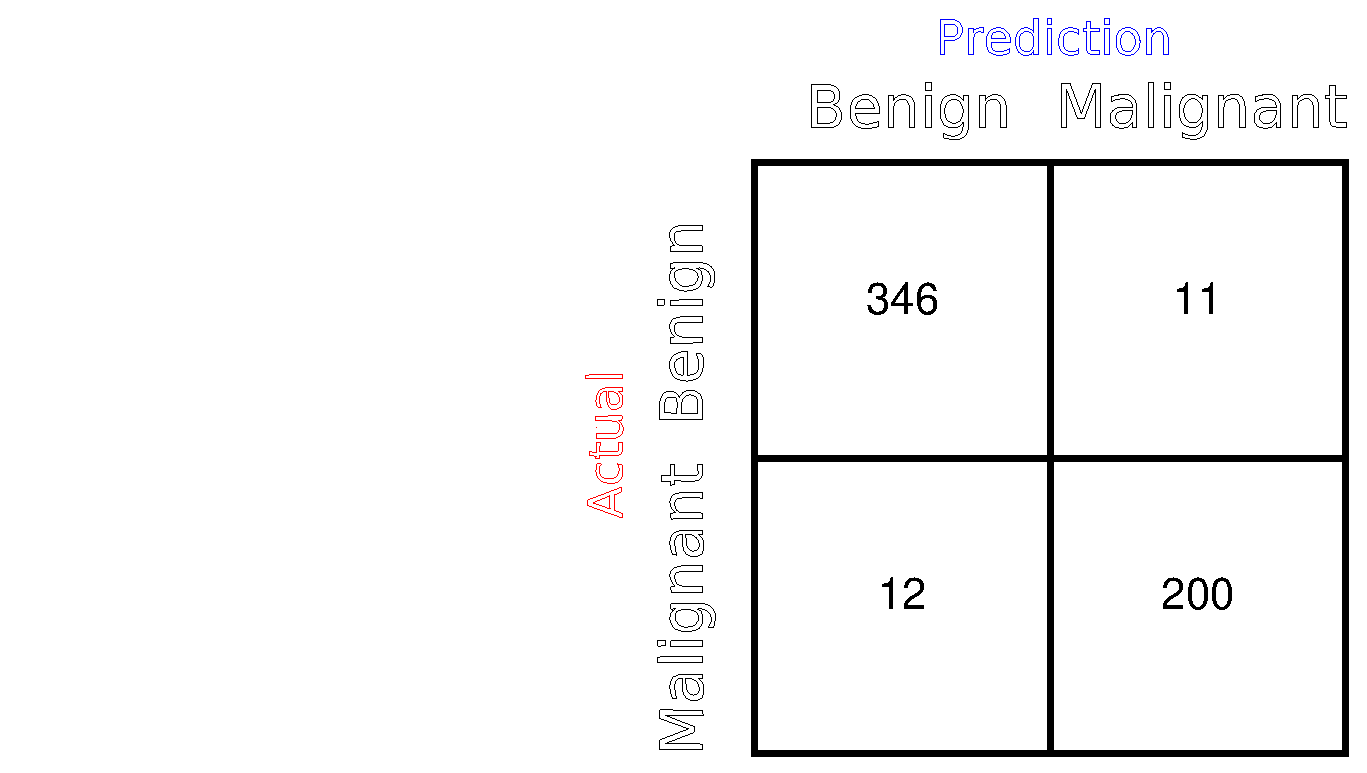
\includegraphics[trim={9cm 0cm 0cm 0cm},clip,scale=0.8]{Figures/SVM_Linear_CM}
	%\includegraphics[trim={0cm 0.5cm 0cm 7cm},clip,scale=0.47]{Figures/BenignMalignantOriginal}  
  \end{center}
  %\vspace{-0.7cm}
  \caption{Confusion matrix for linear kernel SVM model built with all the 30 features and C = 70}
  \label{SVMLinearCM}
\end{figure}

Next we show the performance of SVM model built with the 6 features extracted through K-means. Figure \ref{KSVMLinear} shows the variation of test accuracy, significance and sensitivity with the SVM penalty parameter (C). The highest accuracy (0.81) is achieved when C=80. The confusion matrix for this C value is shown in figure \ref{KSVMLinearCM}. As expected, accuracy of the SVM model built with extracted features is less when compared to the accuracy when all the 30 features are used. However, the time required (see table \ref{LinearTimeTable}) to build the SVM model with extracted features is less when compared with the time taken to build the model with all the 30 features.   
\begin{figure}[H]
  \begin{center}
    \includegraphics[trim={0cm 0cm 0cm 0cm},clip,scale=1]{Figures/KSVM_Linear_Accuracy}
	%\includegraphics[trim={0cm 0.5cm 0cm 7cm},clip,scale=0.47]{Figures/BenignMalignantOriginal}  
  \end{center}
  %\vspace{-0.7cm}
  \caption{Variation of accuracy, sensitivity and specificity with change in SVM penalty parameter (C) for linear kernel SVM model built with the 6 extracted features}
  \label{KSVMLinear}
\end{figure}

\begin{figure}[H]
  \begin{center}
    \includegraphics[trim={9cm 0cm 0cm 0cm},clip,scale=0.8]{Figures/KSVM_Linear_CM}
	%\includegraphics[trim={0cm 0.5cm 0cm 7cm},clip,scale=0.47]{Figures/BenignMalignantOriginal}  
  \end{center}
  %\vspace{-0.7cm}
  \caption{Confusion matrix for linear kernel SVM model built with the 6 extracted features and C = 80}
  \label{KSVMLinearCM}
\end{figure}

\begin{table}[H]
\centering
\begin{tabular}{|l|l|l|l|l|l|l|l|l|l|l|l|l|}
\hline
                                                                                                   & 0.1  & 1    & 10   & 20   & 30   & 40   & 50   & 60   & 70   & 80    & 90  & 100  \\ \hline
\begin{tabular}[c]{@{}l@{}}With all \\ 30 features\end{tabular}      & 2.8  & 11.3 & 47.9 & 49.1 & 64.3 & 79.2 & 94.5 & 67.8 & 71.8 & 71.34 & 74.9 & 75.91  \\ \hline
\begin{tabular}[c]{@{}l@{}}With the \\ 6 extracted features\end{tabular} & 0.03 & 0.04 & 0.04 & 0.05 & 0.04 & 0.05 & 0.05 & 0.06 & 0.05 & 0.06  & 0.06 & 0.07 \\ \hline
\end{tabular}
\caption{Computation time (in sec) of linear kernel SVM}
\label{LinearTimeTable}
\end{table}

\subsubsection{SVM with sigmoid kernel}
Figure \ref{SVMSigmoid} shows the variation of test accuracy with the SVM penalty parameter (C) for sigmoid kernel SVM model which is build with all the 30 features. The figure also shows the variation of sensitivity and specificity. Irrespective of the C value, the accuracy of the model is same. The confusion matrix of the model is shown in figure \ref{SVMSigmoidCM}. The model predicts all the tumors to be malignant. The accuracy of this model is 0.63. Setting a higher C value could increase the accuracy of the model. Note: The accuracy value did not change when the gamma value of sigmoid function was changed.  
\begin{figure}[]
  \begin{center}
    \includegraphics[trim={0cm 0cm 0cm 0cm},clip,scale=1]{Figures/SVM_Sigmoid_Accuracy}
  \end{center}
  \caption{Variation of accuracy, sensitivity and specificity with change in SVM penalty parameter (C) for sigmoid kernel SVM model built with all the 30 features}
  \label{SVMSigmoid}
\end{figure}
\begin{figure}[]
  \begin{center}
    \includegraphics[trim={9cm 0cm 0cm 0cm},clip,scale=0.8]{Figures/SVM_Sigmoid_CM}
  \end{center}
  %\vspace{-0.7cm}
  \caption{Confusion matrix for sigmoid kernel SVM model built with all the 30 features}
  \label{SVMSigmoidCM}
\end{figure}

Next we show the performance of SVM model built with the 6 features extracted through K-means. Figure \ref{KSVMSigmoid} shows the variation of test accuracy, significance and sensitivity with the SVM penalty parameter (C). The highest accuracy (0.79) is achieved when C=80. The confusion matrix for this C value is shown in figure \ref{KSVMLinearCM}. Clearly, the accuracy of the SVM model built with extracted features is more when compared to the accuracy when all the 30 features are used.   
\begin{figure}[]
  \begin{center}
    \includegraphics[trim={0cm 0cm 0cm 0cm},clip,scale=1]{Figures/KSVM_Sigmoid_Accuracy}
	%\includegraphics[trim={0cm 0.5cm 0cm 7cm},clip,scale=0.47]{Figures/BenignMalignantOriginal}  
  \end{center}
  %\vspace{-0.7cm}
  \caption{Variation of accuracy, sensitivity and specificity with change in SVM penalty parameter (C) for sigmoid kernel SVM model built with the 6 extracted features}
  \label{KSVMSigmoid}
\end{figure}

\begin{figure}[]
  \begin{center}
    \includegraphics[trim={9cm 0cm 0cm 0cm},clip,scale=0.8]{Figures/KSVM_Sigmoid_CM}
	%\includegraphics[trim={0cm 0.5cm 0cm 7cm},clip,scale=0.47]{Figures/BenignMalignantOriginal}  
  \end{center}
  %\vspace{-0.7cm}
  \caption{Confusion matrix for sigmoid kernel SVM model built with the 6 extracted features and C = 80}
  \label{KSVMSigmoidCM}
\end{figure}


%******************************************************************
%                         Bibliography or References          
%******************************************************************  
\bibliography{mylit}     

\end{document}

%%% Local Variables: 
%%% mode: latex
%%% TeX-master: t
%%% End: 
